\chapter{Stato dell'arte}
\label{chap:SOA}
\vspace{1cm}
In questo capitolo verrà fornito un esame dello stato dell'arte e verranno presentate 
alcune soluzioni relative al lavoro oggetto di questa tesi.

Nella sezione~\ref{sec:algoritmiProposti} si esaminano i vari approcci proposti 
dagli autori nell'ambito del problema dello scheduling dei task su dispositivi 
riconfigurabili, divisi in algoritmi esatti, trattati nella
sezione~\ref{sec:algoritmiEsatti}, ed euristici, trattati nella
sezione~\ref{sec:algoritmiEuristici}.

La sezione~\ref{sec:osservazioniConclusiveSoA} riepiloga quanto visto in questo capitolo
e fornisce le motivazioni alla base dello sviluppo dell'algoritmo di scheduling
trattato in questa tesi.

\newpage

\section{Algoritmi proposti}
\label{sec:algoritmiProposti}
In questa sezione verranno esaminate diverse soluzioni al problema dello 
scheduling, proposte in altri lavori.

Come anticipato nel capitolo~\ref{chap:intro}, il problema di trovare uno 
schedule di lunghezza minima per un insieme di task in presenza di vincoli di 
risorse appartiene alla classe dei problemi di ottimizzazione 
$\mathcal{NP}$-difficili. Tutte le soluzioni proposte appartengono a una 
tra queste categorie di algoritmi:
\begin{enumerate}
 \item \emph{algoritmi esatti} o \emph{ottimi}, che permettono di ricavare la 
miglior soluzione esistente, tramite l'impiego di opportune strutture matematiche o di 
formulazioni particolari del problema;
 \item \emph{algoritmi euristici}, che in generale portano ad ottenere 
soluzioni sub-ottime. Gli algoritmi euristici si possono suddividere a loro 
volta in sottocategorie in base al loro funzionamento, tra le più importanti 
ricordiamo:
 \begin{itemize}
  \item euristiche basate su una lista, in cui i task vengono schedulati 
secondo l'ordine in cui compaiono nella lista, ordinata per priorità decrescenti;
  \item meta-euristiche, che comprendono algoritmi evolutivi o ispirati al 
comportamento di sistemi presenti in natura.
 \end{itemize}
\end{enumerate}

\begin{figure}[t!]
 \begin{center}
  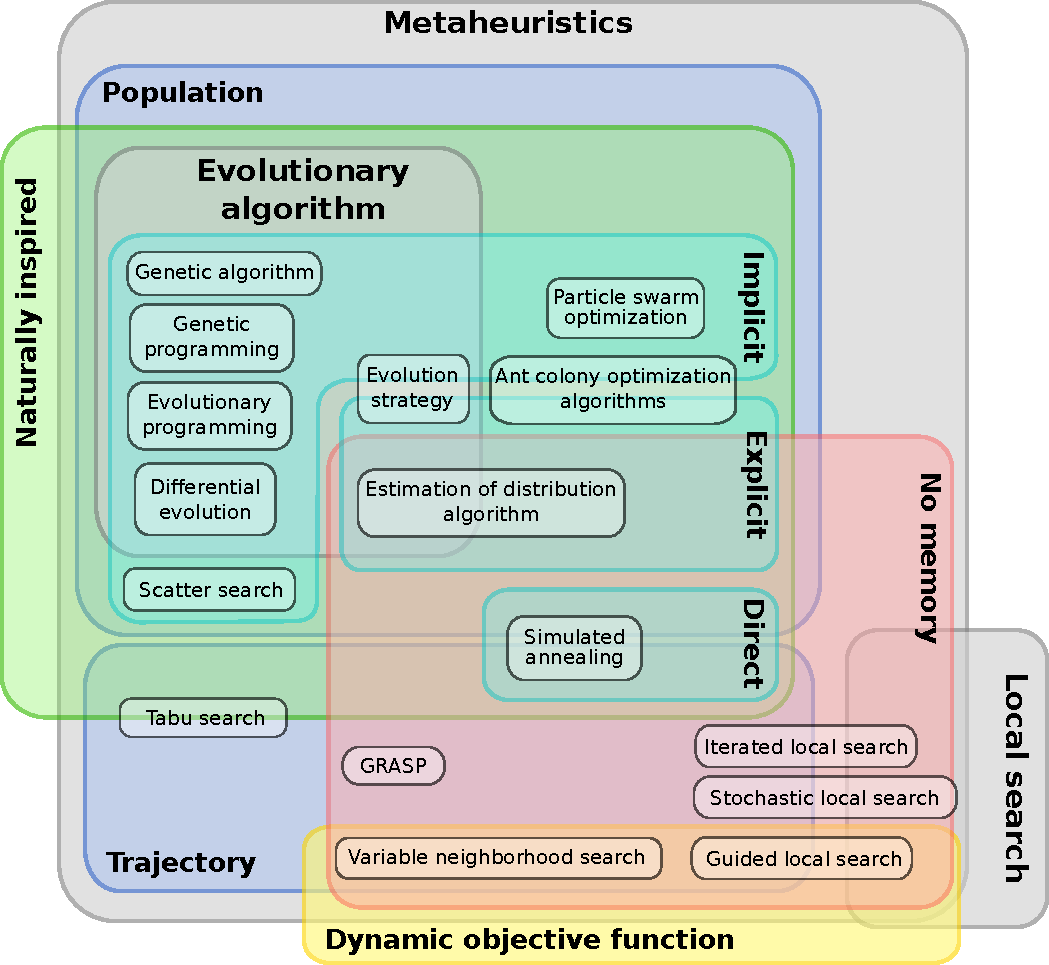
\includegraphics[width=0.7\textwidth]
  {capitoli/figure/cap2/MetaheuristicsClassification.pdf}
  \caption[Classificazione degli algoritmi meta-euristici]{Classificazione delle
  varie categorie di meta-euristiche. Immagine 
realizzata da Johann Dréo \cite{MetaheuristicsClassifications} e tradotta in inglese da Caner Candan.}
\label{fig:metaheuristicsClassification}
 \end{center}
\end{figure}

%%%%%%%%%%
\acrodef{SCOP}{Stochastic Combinatorial Optimization Problem}
%%%%%%%%%%

La classificazione dei diversi tipi di algoritmi meta-euristici è illustrata in 
figura~\ref{fig:metaheuristicsClassification}. Diversi lavori forniscono 
un'analisi di questo tipo di algoritmi euristici, ad esempio lo studio condotto 
da Bianchi et al. \cite{SurveyMetaheuristicSCOP} analizza l'impiego delle 
meta-euristiche per la risoluzione di problemi di ottimizzazione combinatoria stocastica
(in inglese \aclp{SCOP}) o l'analisi effettuata da Blum 
et al. \cite{MetaheuristicCombinatorialOptimization} per problemi di 
ottimizzazione combinatoria.

Il resto della sezione è organizzato come segue: nella
sezione~\ref{sec:algoritmiEsatti} vengono descritte le soluzioni proposte per il 
problema dello scheduling basate su algoritmi esatti; la
sezione~\ref{sec:algoritmiEuristici} presenta invece le soluzioni basate su metodi 
euristici.


\subsection{Algoritmi esatti}
\label{sec:algoritmiEsatti}
Come esposto nell'introduzione a questa sezione, gli algoritmi esatti 
permettono di ottenere la soluzione ottima in assoluto. Un algoritmo esatto, 
applicato a un'istanza di un problema di ottimizzazione combinatoria qual è un
problema di scheduling di task su un numero vincolato di unit\`a computazionali,
definito tramite una formulazione (modello), permette di ottenere lo schedule
caratterizzato dal minimo makespan possibile che rispetti la formulazione. 

A prescindere dal particolare algoritmo utilizzato per risolvere il problema, 
il costo computazionale necessario per giungere a una soluzione è elevato e 
solitamente non polinomiale, a meno di istanze del problema molto particolari e 
in generale difficilmente riscontrabili in casi reali 
\cite{PolynomialCompleteScheduling}.

Nelle prossime sezioni verranno esaminate alcune soluzioni proposte per 
ottenere una soluzione ottima al problema oggetto del lavoro.

\subsubsection{Programmazione lineare}
La programmazione lineare, in inglese \ac{LP} \cite{DantzigLinearProgramming}, è
un metodo matematico che, applicato a un modello con requisiti sotto forma di
vincoli \emph{lineari}, permette di ricavare la soluzione ottima tra tutte le
soluzioni possibili che soddisfano i requisiti. L'ottimalità della soluzione è
determinata in base a una funzione (lineare) detta \emph{funzione obiettivo}.

Il problema è tradotto matematicamente nei termini di un modello, 
caratterizzato da \emph{variabili}, \emph{parametri} e \emph{vincoli}.
La \emph{forma canonica} di un problema di programmazione lineare è espressa 
come:

\begin{align*}
& \text{maximize}   && \mathbf{c}^\mathrm{T} \mathbf{x}\\
& \text{subject to} && A \mathbf{x} \le \mathbf{b},\\
&  && \mathbf{x} \ge \mathbf{0}
\end{align*}

Alternativamente, il problema si può esprimere in maniera equivalente utilizzando
la  \emph{forma standard}:

\begin{align*}
 & \text{maximize}   && \mathbf{c}^\mathrm{T} \mathbf{x}\\
& \text{subject to} && A \mathbf{x} = \mathbf{b}, \\
&  && \mathbf{x} \ge \mathbf{0}
\end{align*}
dove $\mathbf{x}$ rappresenta il vettore di variabili che devono essere 
determinate per trovare la soluzione ottima, $\mathbf{c}$ e $\mathbf{b}$ sono 
vettori di coefficienti costanti e noti, $\mathbf{A}$ è una matrice di 
coefficienti e $(\mathord{\cdot})^\mathrm{T}$ 
rappresenta la trasposizione della matrice/vettore.

È sempre possibile passare dalla forma canonica alla forma standard 
introducendo variabili aggiuntive, dette variabili di \emph{scarto}, che 
permettono di eliminare le disequazioni nei vincoli; le variabili del problema 
che non presentano vincoli di segno possono essere sostituite dalla differenza 
tra due variabili aventi vincoli di segno.

Un problema di programmazione lineare intera, in inglese \ac{ILP}
\cite{ILPBook}, a differenza di un problema di programmazione lineare (come mostrato
nelle precedenti forme), aggiunge un vincolo di interezza per le variabili decisionali
contenute nel vettore $\mathbf{x}$; inoltre, i coefficienti dei vettori $\mathbf{c}$
e $\mathbf{b}$ e della matrice $\mathbf{A}$ sono numeri interi.

I vincoli di interezza possono anche riguardare soltanto alcune delle variabili o 
dei coefficienti, in tal caso si parla di problemi \ac{MILP}.

Nel caso dello scheduling di un task graph, le formulazioni proposte nello 
stato dell'arte presentano modelli con vincoli di interezza per tutte le 
variabili e i coefficienti, sono quindi problemi di programmazione lineare 
intera; i lavori di questo tipo sono descritti nella sezione seguente.


\subsubsection{Formulazioni \acs{ILP}}
Il problema di effettuare lo scheduling di task di un'applicazione per 
l'esecuzione su hardware, anche riconfigurabile, è un tema ampiamente discusso 
in letteratura; molte sono le formulazioni che ricorrono alla programmazione 
lineare intera per trovare una soluzione a questo problema. Spesso, oltre alla 
ricerca di una soluzione per lo scheduling, il modello consente anche di 
determinare un mapping adeguato che minimizzi il tempo di esecuzione finale
dell'applicazione.

Come visto nella sezione~\ref{subsec:faseSchedulingIntro}, infatti, la minimizzazione assoluta 
del tempo di esecuzione può essere ottenuta solamente risolvendo unitamente le 
fasi di mapping, scheduling e floorplanning (per verificare che la soluzione 
sia fisicamente implementabile). In generale, la risoluzione separata delle fasi, in 
particolare la separazione di mapping e scheduling, non porta alla 
minimizzazione assoluta del tempo di esecuzione \cite{AntColonyOptimization}. La scelta tra queste due 
possibilità implica il dover fare un compromesso tra l'accuratezza della 
soluzione, che può non essere la migliore se i problemi sono risolti 
separatamente, e la dimensione dello spazio delle soluzioni possibili, che 
cresce in maniera esponenziale nel caso in cui i problemi si risolvano congiuntamente.
% TODO citazione per frase precedente

\paragraph{Modello \acs{ILP} di Banerjee}
\label{par:BanerjeeILP}
Banerjee et al.~propongono, nel loro 
articolo \cite{BanerjeePhysicalConstraints}, un modello \ac{ILP} che prende in
considerazione una tecnica utilizzata anche in un altro loro lavoro 
\cite{BanerjeeReconfigurationOverhead} nell'ambito delle architetture 
riconfigurabili per ridurre il tempo di esecuzione, dato il considerevole 
over\-head introdotto dalle riconfigurazioni che devono essere eseguite: il 
\emph{configuration prefetching}. Per ridurre il significativo overhead delle 
riconfigurazioni, il configuration prefetching scompone un task in due componenti
separate, di riconfigurazione e di esecuzione. In questo modo si permette al componente 
relativo alla riconfigurazione di essere eseguito separatamente dal task di 
computazione che segue, eliminando le dipendenze dai dati rappresentate dagli 
archi entranti nel task orginale.

\subparagraph{Vincoli di risorse hardware e comunicazioni}
Nello stesso lavoro \cite{BanerjeePhysicalConstraints}, gli autori tengono 
in considerazione i vincoli di piazzamento dei task per verificare che la 
soluzione sia esatta e implementabile: infatti, tutti i task selezionati per 
l'esecuzione su scheda nella fase di partizionamento devono essere 
posizionabili senza violare la disponibilità delle risorse o l'utilizzo esclusivo del 
controllore di riconfigurazione.

\begin{figure}[!hb]
 \begin{center}
  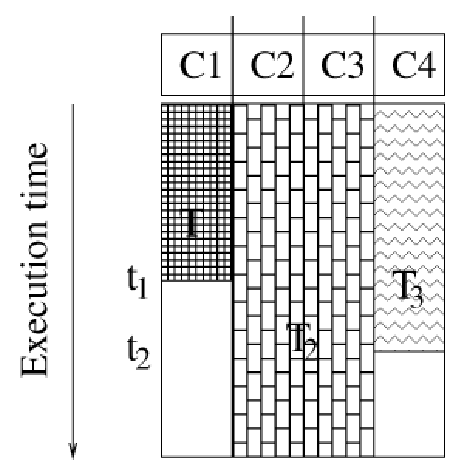
\includegraphics[width=0.3\textwidth]
{./capitoli/figure/cap2/InfeasiblePlacement.pdf}
\caption[Piazzamento ottimo non implementabile]{Esempio di piazzamento ottimo 
ma non implementabile.\footnotemark}
\label{fig:infeasiblePlacement}
 \end{center}
\end{figure}

\footnotetext{Immagine tratta da 
\cite{BanerjeePhysicalConstraints}.}

Un esempio di piazzamento di una soluzione ricavata tramite un algoritmo esatto 
per il partizionamento e lo scheduling di task nel caso di 
architettura con riconfigurazione monodimensionale è rappresentato in 
figura~\ref{fig:infeasiblePlacement}. Si ipotizzi che i requisiti di area per i 
task $T_1$, $T_2$ e $T_3$ siano $1$, $2$, e $1$ colonne, rispettivamente. Inoltre, si
ipotizzi che sia dato il seguente mapping: $\langle T_1, C_1 \rangle$, $\langle
T_2, \{C_2, C_3\} \rangle$ e $\langle T_3, C_4 \rangle$. Dovendo piazzare un nuovo task 
$T_4$, il cui requisito di area è pari a due colonne, un algoritmo che non 
considera le posizioni in cui vengono piazzati i vari task, vedrebbe che al 
tempo $t_2$ vi sono due colonne libere; tuttavia, non essendo $C_1$ e $C_4$ colonne 
adiacenti, il piazzamento non è possibile. Da questa situazione si evince che 
la fattibilità del piazzamento lineare non è garantita dall'utilizzo di un 
algoritmo esatto \cite{BanerjeePhysicalConstraints}.

\subparagraph{Modello e vincoli}
Il modello \ac{ILP} proposto nel loro lavoro prevede quindi la presenza di $n$ 
task che possono avere più implementazioni differenti, sia di tipo SW che HW. 
Nel caso delle implementazioni di tipo HW, ciascuna di esse ha un proprio 
requisito in termini di numero di colonne richieste.\footnote{Ricordiamo che 
poichè l'architettura supporta la riconfigurazione solamente a una dimensione, 
è sufficiente specificare il numero di colonne necessarie per 
un'implementazione.} I vincoli di risorse sono modellizzati considerando un 
processore per l'esecuzione di task SW e fissando un parametro $m$ che 
rappresenta il vincolo sul numero di colonne per il mapping dei task con 
implementazione di tipo HW.

Il configuration prefetching è modellizzato invece creando due variabili 
diverse per ogni task (se la sua implementazione è di tipo HW):
\begin{itemize}
 \item una variabile che rappresenta l'inizio della riconfigurazione;
 \item una variabile che rappresenta l'inizio dell'esecuzione.
\end{itemize}
Per tenere in considerazione i vincoli sulle risorse disponibili e sul 
piazzamento, le variabili che coinvolgono i task mappati su hardware sono 
caratterizzate, oltre a un indice che specifica il task e uno che definisce 
l'istante di tempo, da un indice aggiuntivo che rappresenta la colonna più a 
sinistra del loro mapping. In questo modo è possibile definire vincoli che 
prevengano la sovrapposizione di aree assegnate a task diversi e che rispettino 
in ogni istante la disponibilità di risorse.

\subparagraph{Limitazioni}
La principale limitazione del lavoro proposto in 
\cite{BanerjeePhysicalConstraints} è costituita dal fatto che il modello è 
adatto solo ad architetture che supportano la riconfigurazione parziale a una 
dimensione con un singolo controllore di riconfigurazione, un tipo di 
architettura molto semplice rispetto ai dispositivi utilizzabili oggigiorno,
nei quali è possibile sfruttare l'impiego della riconfigurazione 2D. 
Inoltre, non sono considerate alcune caratteristiche sfruttabili grazie ai 
dispositivi aventi riconfigurazione parziale dinamica, ovvero il \emph{riutilizzo 
dei moduli} ed eventuali tecniche per evitare un'eccessiva \emph{frammentazione} 
delle aree occupate dai task sulla scheda.


\paragraph{Modelli \acs{ILP} di Redaelli} % TODO guardare lavoro di Diana Gohringer su frammentazione
La formulazione \ac{ILP} proposta da Redaelli et al.~\cite{Redaelli1DILP} cerca 
di superare alcune limitazioni che caratterizzano i lavori 
\cite{BanerjeeHwSwPartitioning} e \cite{BanerjeePhysicalConstraints}, visti nel 
precedente paragrafo. % FIXME
Il modello proposto consente infatti di tenere conto delle due tecniche 
sopracitate:
\begin{itemize}
 \item riutilizzo dei moduli, che permette a task diversi che hanno la stessa 
implementazione di essere eseguiti sulla stessa area della scheda (che quindi, 
deve essere configurata soltanto una volta invece che due);
 \item tecniche di anti-frammentazione, che permettono di ridurre la 
frammentazione dello spazio disponibile sulla scheda, così da massimizzare la 
dimensione di aree libere (adiacenti).
\end{itemize}

\subparagraph{Modello \acs{ILP} per architetture riconfigurabili a una 
dimensione}
Il primo modello proposto da Redaelli et al.~in \cite{Redaelli1DILP} è simile 
al modello formulato in \cite{BanerjeePhysicalConstraints}, ma è esteso con 
variabili e costanti che permettono di definire il concetto di riutilizzo dei 
moduli, visto in precedenza. In particolare, è definita una costante 
binaria $a_{ij}$, che assume valore $1$ se i task $i$ e $j$ eseguono la stessa 
azione (quindi il modulo è riutilizzabile); nel modello è inoltre presente una 
variabile binaria $m_i$ che assume valore $1$ se il task $i$ sfrutta un modulo 
riutilizzabile.

I vincoli a cui è soggetto il modello sono formulati in modo da evitare la 
definizione dell'istante iniziale della riconfigurazione di particolari task, 
nel caso in cui tali task sfruttino dei moduli riutilizzabili.

\subparagraph{Modello \acs{ILP} per architetture riconfigurabili a due 
dimensioni}
Il modello proposto da in \cite{Redaelli1DILP} risolve la limitazione 
riguardante la mancata considerazione della possibilità di riutilizzare alcuni 
moduli per guadagnare in termini di overhead di riconfigurazione, ma rimane un 
modello applicabile ad architetture piuttosto datate, dato il supporto limitato
solamente a riconfigurazioni a una dimensione. Per questo, Redaelli et al.~in 
\cite{Redaelli2DILP} propongono una formulazione \ac{ILP} adatta ad 
architetture con riconfigurazione parziale dinamica a due dimensioni.

Il modello è ripreso dal loro lavoro precedente \cite{Redaelli1DILP}, ma 
subisce alcune modifiche atte a supportare la bidimensionalità della 
riconfigurazione e delle aree da piazzare sul dispositivo.

\subparagraph{Descrizione del problema}
In primo luogo, a differenza del precedente lavoro dello stesso autore e 
dei lavori di Banerjee et al.~, cambia la descrizione del problema riguardo alla 
modellazione del dispositivo riconfigurabile. Esso non è più rappresentato 
solamente tramite un insieme di colonne $C = \{c_1,c_2,\dots,c_{\vert C 
\vert}\}$, ma anche tramite un insieme $R = \{r_1,r_2,\dots,r_{\vert R \vert}\}$ 
che ne definisce le righe. Ogni ``cella'' della \ac{FPGA} è quindi identificata 
da una coppia $(r,c)$ con $r \in R$ e $c \in C$, ed è composta da $\rho_u$ 
\acp{CLB}.

\subparagraph{Supporto alla riconfigurazione bidimensionale}
Alcune variabili del modello \ac{ILP} proposte in \cite{Redaelli1DILP} sono 
adattate per supportare la bidimensionalità dell'architettura; gli indici che 
identificano la posizione di un task (o l'occupazione temporale di una certa 
area della scheda) sono quindi due, uno per la colonna più a sinistra e uno per 
la riga più in basso dell'area stabilita per il piazzamento del task.


\paragraph{Limitazioni formulazioni \acs{ILP}}
Oltre alla limitazione dovuta alle potenzialità dell'architettura 
riconfigurabile considerata in \cite{BanerjeePhysicalConstraints}, esiste uno 
svantaggio intrinseco nelle formulazioni di programmazione lineare intera: il 
costo computazionale eccessivo \cite{CombinatorialOptimizationComplexity}. Al
crescere della complessità del modello, il costo in termini di tempo d'esecuzione
del \emph{solver \ac{ILP}} aumenta esponenzialmente.

A titolo esemplificativo della complessità instrinseca dei problemi di programmazione
lineare intera, come riportato in \cite{Redaelli2DILP}, il tempo impiegato per risolvere in 
maniera ottima un'istanza del problema con $10$ task da mappare su una 
\ac{FPGA} con $5$ righe, $5$ colonne e $2$ controllori di riconfigurazione è di 
$39$ giorni, troppo per essere applicabile ad esempi concreti.


\subsubsection{Altri algoritmi ottimi}
% FIXME meglio metterne anche altri, se ci sono...
In questa sezione viene descritto un algoritmo proposto per risolvere in 
maniera ottima il problema di scheduling dei task su dispositivi 
riconfigurabili dinamicamente, che non rientra tra le formulazioni di 
programmazione lineare (intera). L'algoritmo, presentato da Fekete, K\"ohler 
e Teich in \cite{FeketeOptimal}, permette di risolvere due tipi di problemi 
legati allo scheduling:
\begin{enumerate}
 \item trovare il tempo di esecuzione minimo di un problema data una \ac{FPGA} 
con un limite di risorse fissato;
 \item trovare il numero di risorse minimo di cui deve disporre una \ac{FPGA} 
affinchè il tempo di esecuzione sia inferiore a un limite massimo fissato.
\end{enumerate}

Questo lavoro è stato il primo a comprendere la modellazione delle 
comunicazioni tra i vari moduli, includendo il ritardo dovuto alle 
comunicazioni nel tempo di esecuzione dei task.

\begin{figure}[!tb]
 \begin{center}
  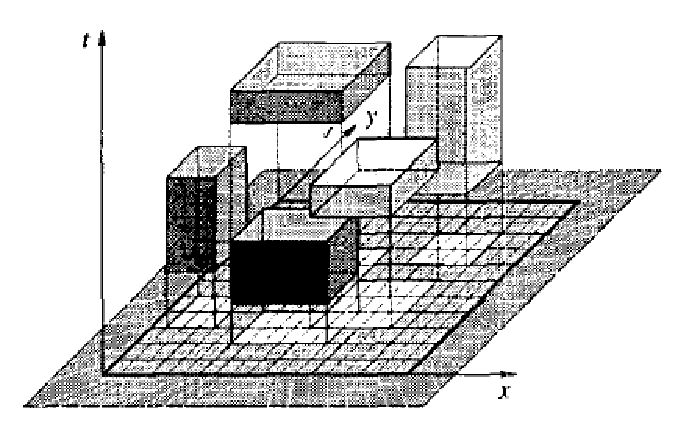
\includegraphics[width=0.5\textwidth]
{capitoli/figure/cap2/BoxModules.pdf}
\caption[Piazzamento dei moduli con rappresentazione tridimensionale]{Esempio 
di piazzamento dei moduli con rappresentazione tridimensionale.\footnotemark}
\label{fig:boxModules}
 \end{center}
\end{figure}

\footnotetext{Immagine tratta da \cite{FeketeOptimal}.}

\paragraph{Modello matematico}
I moduli sono rappresentati nel modello come box di forma tridimensionale, come 
mostrato in figura~\ref{fig:boxModules}. Nella rappresentazione utilizzata, gli 
assi $x$ e $y$ identificano le due dimensioni spaziali (per il piazzamento del 
modulo sulla scheda), mentre l'asse $t$ identifica la dimensione temporale 
(ovvero il tempo di esecuzione). È importante quindi che i moduli vengano 
piazzati dentro all'area disponibile e non siano sovrapposti nel caso di esecuzione
simultanea.

L'idea alla base del metodo è di trattare i task come scatole tridimensionali e 
i possibili schedule \emph{feasible} come disposizioni di tali scatole che 
soddisfano i vincoli di precedenza.

\paragraph{Limitazioni}
La principale limitazione del modello proposto in \cite{FeketeOptimal} è 
l'assunzione che ci sia un numero potenzialmente infinito di controllori di 
riconfigurazione, un'ipotesi che toglie realismo nell'applicazione del metodo 
in scenari concreti. Infatti, non esistono e non esisteranno mai architetture
riconfigurabili con un numero arbitrario di controllori, perch\`e ci\`o comporterebbe
una contention sulla memoria da cui si recupera il bitstream.
Per questo motivo, l'algoritmo \cite{FeketeOptimal} rischia di sottostimare in maniera
non trascurabile il makespan dell'applicazione; l'overhead introdotto dalle riconfigurazioni
infatti non è trascurabile e l'esecuzione di un numero considerevole di riconfigurazioni 
diventa inevitabilmente un collo di bottiglia in casi reali (senza ipotizzare un numero
potenzialmente infinito di controllori), penalizzando il tempo di 
esecuzione.


\subsection{Algoritmi euristici}
\label{sec:algoritmiEuristici}
Dopo aver fornito una panoramica degli algoritmi esatti vengono ora esaminate 
alcune soluzioni euristiche presenti nello stato dell'arte. In generale, le 
soluzioni prodotte da algoritmi euristici per un problema non sono ottime 
(esatte). Si ricorre all'impiego di algoritmi euristici qualora altri metodi 
esatti non possano essere applicati oppure siano troppo lenti nel risolvere il 
problema; in questi casi, si deve sempre trovare un compromesso tra la 
qualità della soluzione trovata e il tempo impiegato per giungere a quella 
soluzione.

Le euristiche si classificano in base al modo di ricercare o costruire una soluzione 
approssimata.
%%%%%%%%%%%%% FIXME controllare
Uno stesso problema può essere risolto utilizzando più di una 
euristica, ma non è garantito che tutte le euristiche applicate a uno stesso 
problema restituiscano la stessa soluzione.

Esistono euristiche specifiche per risolvere determinate classi di problemi che 
si distinguono in base al grado di approssimazione delle soluzioni trovate. 
In tal senso, un'euristica potrebbe performare meglio di altre, se applicata 
allo stesso problema.
%%%%%%%%%%%%%

\subsubsection{Partizionamento HW-SW}
Tra l'ampia varietà di algoritmi euristici proposti nello stato dell'arte per 
risolvere il problema di scheduling dei task, alcuni di questi algoritmi 
considerano come ulteriore obiettivo il partizionamento tra task hardware e 
task software. Ad esempio, Mei et al.~propongono in 
\cite{MeiPartitioningScheduling} un approccio basato sulla combinazione di un 
algoritmo genetico standard\footnote{Gli algoritmi genetici appartengono alle 
meta-euristiche di tipo evolutivo ispirate al funzionamento di sistemi presenti 
in natura, come rappresentato in figura~\ref{fig:metaheuristicsClassification}.}
con un'euristica basata su lista di priorità. Il loro metodo è adatto ad
architetture riconfigurabili dinamicamente e risolve, oltre allo scheduling,
anche il partizionamento dei task che compongono l'applicazione.

Per la fase di partizionamento, nella quale viene deciso il tipo 
di implementazione da utilizzare per ogni task (software o hardware), si usa un 
algoritmo genetico che al suo interno esegue lo scheduling come subroutine per 
effettuare la valutazione di una determinata partizione.

% TODO scendere più nel dettaglio (rappresentazione cromosomi, fitness 
% function, operatori utilizzati)

L'overhead introdotto dalla riconfigurazione parziale è tenuto in 
considerazione e aggiunto al tempo di computazione dei task; tuttavia, non 
vengono impiegate tecniche per mascherare il tempo di riconfigurazione (come il 
\emph{configuration prefetching}) e il collo di bottiglia causato dalle 
limitazioni del controllore della riconfigurazione, che impongono 
riconfigurazioni non sovrapposte nel tempo.


\subsubsection{\acl{EPR} e \acl{IR}}
Jeong et al.~propongono in \cite{JeongHWSWCosynthesis} due metodi diversi per 
risolvere problemi di \emph{hardware-software cosynthesis}: una formulazione 
\ac{ILP} per ricavare una soluzione esatta e una euristica.

L'algoritmo euristico si basa sull'euristica iterativa proposta da 
Fiduccia-Mattheyses per risolvere il problema del bipartizionamento di un
ipergrafo \cite{FiducciaMattheyses}.

% TODO parlare di euristica iterativa KLFM, move and lock, ecc.

In entrambi i metodi (\ac{ILP} ed euristica) vengono incorporati due concetti 
nel calcolo del trade-off del partizionamento hardware-software, per meglio 
sfruttare le capacità di riconfigurazione della \ac{FPGA} su cui dev'essere
eseguita l'applicazione:
\begin{itemize}
 \item \ac{EPR}, rappresenta il concetto di \emph{configuration prefetching};
 \item \ac{IR}, che consente di ridurre la quantità di dati necessari per la 
riconfigurazione, ovvero la dimensione del \emph{bitstream}; partendo da task 
che condividono parzialmente i dati necessari alla loro configurazione è 
possibile configurare in maniera incrementale soltanto le porzioni dei 
moduli che differiscono tra di loro, a condizione che tra le esecuzioni non si 
verifichino riconfigurazioni dell'intera area.
\end{itemize}

\subparagraph{Limitazioni}
Nonostante le precedenti strategie adottate per ridurre l'impatto dell'overhead 
introdotto dalle riconfigurazioni, la maggior limitazione del lavoro proposto 
in \cite{JeongHWSWCosynthesis} consiste nella mancata considerazione dei 
vincoli e dei limiti fisici imposti dall'architettura target. Pertanto, le 
soluzioni trovate potrebbero non essere fisicamente implementabili, pur essendo 
ottime o sub-ottime (nel caso si usi l'euristica).

\subsubsection{Euristica di Banerjee}
Nel lavoro di Banerjee et al.~\cite{BanerjeePhysicalConstraints}, lo stesso in 
cui è presentata la formulazione \ac{ILP} vista nella sezione~\ref{par:BanerjeeILP}, è 
descritto anche un metodo euristico per la risoluzione dei problemi di 
partitionamento, scheduling e piazzamento fisico dei task rispettando i vincoli 
architetturali.

L'euristica proposta in \cite{BanerjeePhysicalConstraints} cerca di porre 
rimedio alle limitazioni del metodo proposto in \cite{JeongHWSWCosynthesis} 
presentate nel paragrafo precedente, considerando il piazzamento dei moduli 
come parte integrante dell'algoritmo di partizionamento e scheduling.

\acrodef{BRAM}{Block Random Access Memory}

\subparagraph{Approccio}
Il loro approccio si basa su un'euristica di tipo iterativo, come formulata da 
Kernighan-Lin \cite{KernighanLin} e Fiduccia-Mattheyses 
\cite{FiducciaMattheyses}. Per tenere conto di possibili ottimizzazioni 
effettuate dai compilatori, è supportata l'esistenza di più di una 
implementazione per ogni task.

Come nel lavoro \cite{JeongHWSWCosynthesis}, la parte di valutazione di una 
``mossa'' nel partizionamento viene effettuata da uno scheduler list-based. La 
priorità dei task è calcolata come combinazione lineare di una serie di 
metriche, come l'istante al più presto di avvio, l'istante al più presto di 
fine e il requisito in termini di area (colonne) occupata dal modulo.


\subparagraph{Eterogeneità delle risorse}
Un'altra importante caratteristica dell'euristica proposta, naturale 
conseguenza del tenere in considerazione i vincoli hardware durante il 
piazzamento fisico dei moduli, è la possibilità di estendere l'approccio per 
supportare l'eterogeneità di risorse,\footnote{L'eterogeneità delle risorse 
consiste nell'avere delle risorse aggiuntive incorporate sul die, ad esempio 
memorie a blocchi (\acs{BRAM}), \acp{DSP}, moltiplicatori. Ciò consente ai 
designer di utilizzare le risorse aggiuntive presenti, senza bisogno di 
implementare manualmente tutte le funzionalità necessarie. Le risorse 
incorporate sono anche chiamate processori hardcore, in contrapposizione ai 
processori softcore, che rappresentano unità computazionali implementate usando 
la logica riconfigurabile messa a disposizione dall'\ac{FPGA}} un fattore 
chiave per l'incremento di prestazioni delle applicazioni implementate su 
\ac{FPGA} moderne; dato che le risorse eterogenee sono disponibili soltanto in 
posizioni ``prefissate'' della scheda, l'attenzione nella scelta dell'area da 
assegnare a un modulo risulta un fattore determinante per l'incremento delle 
performance dell'applicazione da accelerare.

\subparagraph{Limitazioni}
Nonostante la velocità di esecuzione dell'euristica proposta,\footnote{Gli 
autori affermano che task graph aventi una dimensione di centinaia di nodi 
completano le fasi di partitioning, scheduling e placement nel giro di pochi 
minuti.} le limitazioni che caratterizzano questo metodo sono le stesse della 
formulazione \ac{ILP} proposta nello stesso articolo. L'architettura target
considerata è dotata di riconfigurazione parziale dinamica, ma soltanto a una 
dimensione; inoltre, il riutilizzo dei moduli per guadagnare tempo di esecuzione 
non viene mai considerato.

\paragraph{PARLGRAN}
Banerjee et al.~introducono PARLGRAN in un lavoro seguente 
\cite{BanerjeePARLGRAN}, come soluzione migliorata ai problemi di 
scheduling e placement in presenza di vincoli di risorse. L'obiettivo di 
PARLGRAN è selezionare il miglior livello di granularità di parallelismo dei 
dati, per task che operano su dati parallelizzabili. Allo scopo di considerare 
l'overhead di riconfigurazione e possibili problemi nel piazzamento dei task, 
vengono utilizzate due tecniche:
\begin{itemize}
 \item \emph{simple fragmentation reduction};
 \item \emph{exploiting slack in reconfiguration controller}.
\end{itemize}
La prima tecnica consiste nell'evitare il più possibile che due task siano 
piazzati in maniera adiacente sulla scheda; il piazzamento del secondo task 
avviene infatti su lato opposto della scheda, se possibile. In questo modo è 
possibile sfruttare lo spazio libero per riconfigurare ed eseguire task con un 
requisito di area maggiore.

\begin{figure}[t]
\begin{minipage}[b]{0.4\textwidth}
 \begin{center}
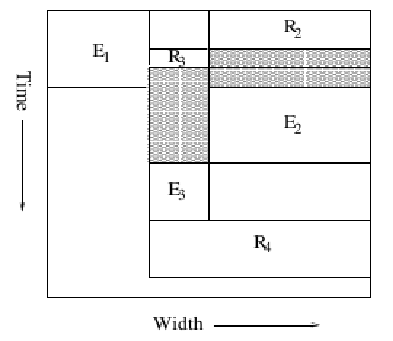
\includegraphics[width=\linewidth]{capitoli/figure/cap2/SlackRecController1.pdf}
\subcaption{Più frammentazione}
\label{fig:slackRecController1}
 \end{center}
\end{minipage}
\hfill
\begin{minipage}[b]{0.4\textwidth}
 \begin{center}
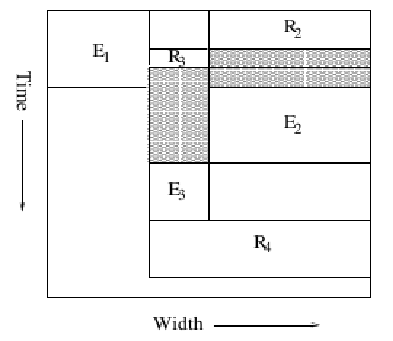
\includegraphics[width=\linewidth]{capitoli/figure/cap2/SlackRecController1.pdf}
\subcaption{Meno frammentazione}
\label{fig:slackRecController2}
 \end{center}
\end{minipage}
\caption[Applicazione della tecnica exploiting slack in reconfiguration 
controller]{Applicazione della tecnica \emph{exploiting slack in reconfiguration 
controller}.\footnotemark}
\label{fig:slackRecController}
\end{figure}


La seconda tecnica, usata come metodo di ottimizzazione locale per ridurre la 
frammentazione, permette di trarre vantaggio da eventuali periodi di inattività 
tra il termine di una riconfigurazione e l'esecuzione del task relativo. Un 
esempio di applicazione di tale tecnica è mostrato in figura~\ref{fig:slackRecController}.
Nella figura~\ref{fig:slackRecController1} si può 
vedere come vi sia un tempo morto tra la riconfigurazione del task $T3$ e la sua 
esecuzione, che rallenta l'inizio della riconfigurazione del task $T4$. Il task 
$T3$ può quindi essere piazzato in una diversa posizione, come raffigurato in 
figura~\ref{fig:slackRecController2}, consentendo alla riconfigurazione del task 
$T4$ di partire anticipatamente, senza che l'istante di fine esecuzione di $T3$ 
sia influenzato dallo spostamento.

\footnotetext{Immagine tratta da \cite{BanerjeePARLGRAN}.}


L'utilizzo congiunto delle due tecniche sopra descritte permette di guadagnare 
in termini di makespan dello schedule finale e di produrre quindi soluzioni di 
miglior qualità, sempre con l'obiettivo principale di integrare i vincoli di 
risorse e garantire la generazione di soluzioni fisicamente implementabili.

%%% TODO parlare dello static pruning?

\subparagraph{Limitazioni di PARLGRAN}
La principale limitazione di PARLGRAN, oltre al mancato supporto di 
architetture con riconfigurazione parziale dinamica bidimensionale, consiste 
nella mancata considerazione della gestione della memoria nel caso di task 
paralleli che lavorano su parti diverse di uno stesso insieme di dati. Inoltre, 
non è presente nessuna valutazione quantitativa della memoria disponibile per 
i task; questo potrebbe diventare un problema nel caso in cui si debbano 
risolvere particolari istanze.


\subsubsection{Napoleon}
\emph{Napoleon} è un algoritmo euristico presentato da Redaelli et al.~in 
\cite{Redaelli2DILP}. Le sue caratteristiche distintive sono la capacità di 
supportare architetture riconfigurabili bidimensionali e la possibilità di 
sfruttare alcune tecniche viste in precedenza in diversi altri lavori e altre 
tecniche nuove: \emph{configuration prefetching}, \emph{riutilizzo dei moduli} e 
tecniche di \emph{anti-frammentazione}.

In particolare, Napoleon adotta la tecnica chiamata \emph{limited 
deconfiguration};\footnote{La deconfigurazione limitata consiste nel tenere 
tutti i moduli configurati sull'\ac{FPGA} finchè altri task non richiedono le 
loro risorse.} grazie a questa si può incrementare la possibilità di 
un eventuale riutilizzo dei moduli.

Oltre ad applicare la deconfigurazione limitata, Napoleon si basa sul criterio 
di \emph{farthest placement},\footnote{La tecnica di \emph{farthest placement} 
mira a piazzare fisicamente il task nella zona che abbia area sufficiente per 
contenere il task e sia il più distante possibile dal centro della scheda.} per 
la fase di piazzamento dei task. Questo criterio ha come scopo il favorire il 
piazzamento di task futuri: è infatti più facile piazzare moduli con grandi 
requisiti di area al centro della scheda.

L'euristica Napoleon supporta più di un controllore di riconfigurazione, 
laddove l'architettura obiettivo possegga queste caratteristiche. Dai risultati 
dei test sperimentali risulta che nel caso vengano utilizzati due 
riconfiguratori, l'algoritmo ha calcolato la soluzione ottima in $7$ istanze su 
$10$ benchmark diversi. In generale, ad un aumento del numero di 
riconfiguratori disponibili corrisponde un aumento della qualità della 
soluzione generata, in quanto è possibile sfruttare maggiormente tecniche di 
ottimizzazione quali ad esempio il configuration prefetching.

\subparagraph{Limitazioni}
Nonostante la qualità dei risultati generati, il tempo di esecuzione più che 
ragionevole e le tecniche di ottimizzazione utilizzate, il limite di Napoleon è 
la mancata considerazione esplicita delle comunicazioni tra i task di 
computazione. Inoltre, l'algoritmo euristico proposto non considera la 
possibilità di avere task con implementazioni software che possano essere 
eseguiti su uno o più processori general purpose, oltre ai task accelerati in 
hardware.


\subsubsection{\acl{ACO}}
L'ultimo algoritmo euristico presentato in questa disamina dello stato 
dell'arte è un algoritmo meta-euristico, il cui funzionamento è ispirato alle 
dinamiche di sistemi naturali, l'\ac{ACO} \cite{AntSystem}. Nella fattispecie, 
l'algoritmo cerca di riprodurre il procedimento seguito da una colonia di 
formiche alla ricerca di cibo; la colonia deve poter giungere al cibo seguendo 
il percorso più breve, che rappresenta una soluzione (subottima) trovata.

L'algoritmo \ac{ACO}, una meta-euristica di recente sviluppo, è stato inizialmente 
utilizzato per risolvere il problema del commesso viaggiatore (\acs{TSP}) 
\cite{AntSystem} e poi esteso anche ad altri problemi di ottimizzazione 
combinatoria.

\paragraph{Funzionamento}
Quando una colonia va alla ricerca di cibo, tutte le formiche partono dalla 
colonia seguendo direzioni casuali, lasciando una traccia di 
\emph{feromone}\footnote{Il feromone è una sostanza emessa da alcuni esseri 
viventi con funzione di segnalare qualcosa agli individui riceventi 
della stessa specie: una traccia, un pericolo, una modificazione 
comportamentale per il ricevente.} sul loro cammino. La traccia di feromone 
evapora con il tempo, ma il percorso più breve dalla colonia al cibo conterrà 
sempre più feromoni, attirando le altre formiche su quel percorso invece che su 
cammini più lunghi.

In ottica stocastica, la quantità di feromone rappresenta la probabilità, per 
ciascuna decisione, di giungere a una buona soluzione. All'inizio 
dell'algoritmo, la matrice dei feromoni è inizializzata con valori uniformi 
(tutte le decisioni hanno uguale probabilità). Seguendo il modello naturale, un 
certo numero di procedure di generazione delle soluzioni (formiche) viene 
lanciato. Nella fase di decisione, viene assegnata una probabilità ad ogni 
scelta possibile, funzione della posizione corrente nel processo decisionale, 
della destinazione da raggiungere, di una euristica locale calcolata ogni volta 
che la probabilità è generata e di una euristica globale. La formula per il 
calcolo della probabilità è la seguente:
\begin{equation}
 p_{x,y} = \frac{[\tau_{x,y}]^{\alpha}\cdot[\eta_{x,y}]^{\beta}}{\sum_{l \in 
\Omega_{x}}[\tau_{x,l}]^{\alpha}\cdot[\eta_{x,l}]^{\beta}}
\end{equation}
dove $x$ è la posizione corrente nel processo decisionale, $y$ è la 
destinazione della ricerca, $\eta$ è l'euristica locale legata al problema e 
$\tau$ è l'euristica globale determinata dal feromone. $\alpha$ e $\beta$ 
rappresentano i pesi che vengono dati alle due euristiche e che influenzano il 
comportamento della formica nel processo decisionale. $\Omega_x$ è l'insieme che 
contiene tutte le scelte possibili al passo corrente $x$. Alla fine di ogni 
processo decisionale, avendo ottenuto diverse soluzioni, la matrice dei 
feromoni è aggiornata con la formula
\begin{equation}
 \tau_{x,y} = (1-\rho)\cdot \tau_{x,y} + \epsilon
\end{equation}
dove $\rho$ è il \emph{fattore di evaporazione} del feromone, mentre $\epsilon$ 
rappresenta un coefficiente correttivo di rinforzo che evita di penalizzare 
tramite l'evaporazione anche le scelte migliori.


\paragraph{Applicazioni}
Ferrandi et al.~propongono in \cite{AntColonyOptimization} un algoritmo basato 
sull'euristica \ac{ACO} per effettuare mapping e scheduling di task e 
comunicazioni su un sistema \ac{MPSoC} eterogeneo. Il loro approccio considera 
la presenza di più \emph{implementation point}, che rappresentano le diverse 
implementazioni possibili per i task che compongono l'applicazione. Oltre a 
questo, l'architettura è considerata formata da componenti di computazione e 
componenti di comunicazione; ad ogni componente dell'architettura è associato 
un insieme di risorse \emph{rinnovabili} (ad esempio risorse che possono essere 
riconfigurate dopo l'utilizzo) e \emph{non rinnovabili} (nel caso contrario).
Grazie a questa formulazione l'algoritmo si adatta a diversi tipi di 
architetture; inoltre, la differenza tra risorse rinnovabili e non modellizza 
sia processori general purpose, risorse rinnovabili per definizione, sia core 
implementati su logica riconfigurabile, rinnovabili tramite la riconfigurazione.

% TODO manca AHS 2013


\section{Osservazioni conclusive}
\label{sec:osservazioniConclusiveSoA}
In questo capitolo è stato innanzitutto presentato il progetto europeo \ac{FASTER},
il cui obiettivo è fornire un framework ai designer per l'esecuzione di applicazioni
su diverse architetture riconfigurabili, considerando la riconfigurazione parziale come
concetto esplicito nel design del sistema per migliorare le prestazioni dell'applicazione.

La toolchain è composta da diverse parti, sviluppate dai partner del progetto,
e si occupa della gestione nella maniera più automatizzata possibile dell'analisi
del codice, delle possibilità di (micro)riconfigurazione, delle fasi di partitioning,
scheduling e floorplanning dei moduli che compongono l'applicazione.

Sono stati presentati, inoltre, alcuni algoritmi ideati da vari autori per risolvere
il problema di scheduling (congiuntamente oppure separatamente rispetto a
partitioning/mapping). In particolare, sono stati descritti gli algoritmi esatti e quelli
euristici, in due sezioni separate, con relative limitazioni.

Il flusso di esecuzione della toolchain di \ac{FASTER} prevede l'invocazione del tool di baseline
scheduling statico come componente esterno, chiamato dall'algoritmo di esplorazione dello spazio
di design per il mapping; il componente di scheduling effettua la valutazione di una particolare
metrica, la stima del tempo di esecuzione totale dello schedule calcolato. Poichè la fase
di mapping è implementata come un algoritmo esplorativo evolvibile che chiama lo scheduler
baseline come componente di valutazione della metrica riguardante il makespan, l'algoritmo di
scheduling deve necessariamente essere veloce, per non rallentare eccessivamente l'esplorazione.

Alla luce di queste considerazioni, si è deciso di sviluppare un algoritmo basato su
un'euristica, per soddisfare i requisiti di velocità. L'algoritmo di scheduling non
dovrebbe essere un'euristica esplorativa, quanto più un algoritmo veloce di tipo list-based,
con una funzione di calcolo delle priorità che gli consenta di essere sufficientemente preciso,
restituendo quindi degli schedule di buona qualità.

% TODO FIXME delta rispetto agli altri algoritmi presentati!
